\documentclass[11pt]{article}
% Shared preamble of the two technical papers (docs/paper). Compile with latexmk -pdf <paper>.tex
\usepackage[T1]{fontenc}
\usepackage[utf8]{inputenc}
\usepackage{lmodern}
\usepackage[a4paper,margin=25mm,headheight=14pt]{geometry}
\usepackage{microtype}
\usepackage{amsmath,amssymb,bm}
\usepackage{graphicx}
\usepackage{booktabs,tabularx,multirow}
\usepackage[detect-all,per-mode=symbol]{siunitx}
\usepackage{xcolor}
\usepackage{tikz}
\usetikzlibrary{arrows.meta,positioning,fit,calc,shapes.geometric,backgrounds}
\usepackage{caption,subcaption}
\usepackage{enumitem}
\usepackage{algorithm}
\usepackage{algpseudocode}
\usepackage{authblk}
\usepackage{fancyhdr}
\usepackage[numbers,sort&compress]{natbib}
\usepackage[colorlinks=true,linkcolor=blue!50!black,citecolor=blue!50!black,urlcolor=blue!50!black]{hyperref}
\usepackage[capitalise,noabbrev]{cleveref}

\definecolor{lrred}{HTML}{C8102E}
\definecolor{cA}{HTML}{2A78D6}
\definecolor{cB}{HTML}{EB6834}
\definecolor{cC}{HTML}{1BAF7A}
\definecolor{boxbg}{HTML}{F3F4F6}

\captionsetup{font=small,labelfont=bf,margin=4pt}
\setlist{itemsep=2pt,topsep=3pt}
\sisetup{group-minimum-digits=4}
\numberwithin{equation}{section}

\pagestyle{fancy}
\fancyhf{}
\renewcommand{\headrulewidth}{0.3pt}
\fancyfoot[C]{\thepage}

\newcommand{\code}[1]{\texttt{\small #1}}
\newcommand{\vect}[1]{\bm{#1}}
\renewcommand{\Affilfont}{\small\itshape}

% TikZ styles for the block diagrams
\tikzset{
  blk/.style={draw=black!60, fill=boxbg, rounded corners=2pt, align=center, font=\footnotesize, inner sep=4pt, minimum height=8mm},
  grp/.style={draw=black!35, dashed, rounded corners=3pt, inner sep=5pt},
  grplab/.style={font=\scriptsize\itshape, text=black!60},
  arr/.style={-{Stealth[length=2mm]}, semithick, black!70},
  darr/.style={{Stealth[length=2mm]}-{Stealth[length=2mm]}, semithick, black!70},
}


\fancyhead[L]{\small Performance Lab: lap time simulation of the LR26}
\fancyhead[R]{\small Lions Racing Team}

\title{\textbf{Performance Lab: Quasi-Steady-State and Transient Lap Time Simulation\\for the Lions Racing LR26 Formula Student Vehicle}\\[4pt]
\large Vehicle model, solver, competition scoring, sensitivity and energy analysis, and log correlation}
% Authors: edit as appropriate.
\author{Lions Racing Team -- Performance and Driverless Divisions}
\affil{Formula Student Germany}
\date{Technical report, November 2026}

\begin{document}
\maketitle
\thispagestyle{fancy}

\begin{abstract}
\noindent
The Performance Lab is a stand-alone tool for evaluating the vehicle performance of the Lions Racing LR26. It
runs on any Windows computer with Python, without the driverless simulator's ROS or GPU stack. Its core is a
line-by-line port of the Performance department's MATLAB quasi-steady-state (QSS) lap time simulation (LR26
LapSim). The vehicle model has quasi-static longitudinal and lateral load transfer, load-sensitive tyre
potentials, a friction ellipse with cornering priority, a torque- and power-limited powertrain, and aerodynamic
drag and downforce. The solver computes a curvature-limited speed, then forward and backward integration passes
on the squared speed, all on the competition's FSA~2025 tracks, and scores the result with the competition
formulas.

Around this core, the tool adds:
\begin{itemize}
  \item one-at-a-time sensitivities, one- and two-parameter sweeps and setup comparisons;
  \item an energy decomposition of the endurance lap and the endurance power cap that meets a battery budget;
  \item ggV diagrams;
  \item a transient lap, driven by the driverless simulator's dynamic vehicle model and reference driver;
  \item correlation of logged or reference speed traces against the simulated lap, and motor efficiency maps
        identified from inverter logs.
\end{itemize}
The port reproduces the MATLAB results to within \SI{0.005}{ms} over 85 parameter values and four events. A full
four-event evaluation takes \SI{0.3}{s}. The baseline LR26 scores 164.35 dynamic-event points. Friction (5.6
points per \%) and mass (2.5 points per \%, 0.86 points per kg) dominate the sensitivities. A gear ratio of about
19.3 would gain 21 points. For a \SI{5}{kWh} endurance budget, the power cap is \SI{15.3}{kW}. The transient lap is
3.5--8\,\% slower than QSS, which quantifies the margin a real driver or controller needs.
\end{abstract}

\noindent\textbf{Keywords:} lap time simulation; quasi-steady-state; Formula Student; vehicle dynamics; sensitivity
analysis; energy management; data correlation.

\tableofcontents
\newpage

%=====================================================================================================
\section{Introduction}
%=====================================================================================================
Formula Student design decisions trade points against each other: mass against downforce, gear ratio against top
speed, power against endurance energy. The Performance department turns these trade-offs into numbers with a lap
time simulation (LTS). The LTS predicts the time of each dynamic discipline (acceleration, skidpad, autocross,
endurance) and converts the times into competition points. The LR26 LTS was written in MATLAB. It encodes the
team's vehicle description (\code{lr26\_params.m}) and the competition definition, with tracks, driver
utilisation and scoring (\code{competition\_fsa2025.m}).

Two needs motivated the Performance Lab:
\begin{enumerate}
  \item \textbf{One model.} The driverless simulator~\cite{dvsim} should use the same car as the LTS. That required
        a Python port of the LTS that is identical to MATLAB, not an approximation of it.
  \item \textbf{One tool.} The performance studies (sensitivities, sweeps, energy, correlation) should be available
        to every member of the department, without MATLAB licences, WSL, ROS or a GPU. They should also go
        further than a steady-state model, quantifying what transient vehicle behaviour costs.
\end{enumerate}

\paragraph{Contributions.}
\begin{itemize}
  \item A verified port of the LR26 QSS LTS: vehicle model, solver, track processing and scoring
        (\cref{sec:model,sec:solver,sec:tracks,sec:scoring}).
  \item Analysis methods with precise definitions: sensitivities, sweeps, setup comparison, energy decomposition,
        power cap optimisation and ggV (\cref{sec:studies,sec:energy}).
  \item A transient lap that couples the same vehicle limits to a dynamic single-track model and a
        path-following driver, with a method to close inconsistent curvature tables (\cref{sec:transient}).
  \item Minimum-time optimal control with point-mass, single- and double-track models, a comparison of all
        methods, and a Monte-Carlo robustness study (\cref{sec:methods}).
  \item Log correlation on distance with offset search, and motor-efficiency identification from inverter logs
        (\cref{sec:logs}).
  \item A self-contained web application (\cref{sec:software}) and its verification (\cref{sec:verification}).
\end{itemize}

%=====================================================================================================
\section{Background}\label{sec:background}
%=====================================================================================================
Lap time simulation methods range from steady-state ``apex speed'' methods, through quasi-steady-state (QSS)
methods, to transient optimal control~\cite{siegler2000,brayshaw2005,casanova2000}.

QSS methods treat the car as a sequence of steady states along a fixed path. At every point, the speed is limited
by the cornering capability at the local curvature. Between corners, the car accelerates or brakes at the limit
the tyres, the powertrain and the aerodynamics allow. Siegler \emph{et al.}~\cite{siegler2000} found QSS lap times
within a few percent of transient simulations, at a tiny fraction of the cost. That makes QSS the standard tool for
parameter studies.

Transient methods add yaw, load-transfer and actuator dynamics. They require either a driver model or the solution
of a minimum-time optimal control problem~\cite{casanova2000}. Optimal control gives the theoretical best lap. A
driver model gives a lap that a closed-loop controller can actually achieve, which is the relevant number for a
driverless car.

The tyre model follows the friction-ellipse idea of combined slip~\cite{pacejka2012}, and the vehicle equations
follow standard texts~\cite{milliken1995,rajamani2012}.

%=====================================================================================================
\section{Vehicle model}\label{sec:model}
%=====================================================================================================
The vehicle is a point mass on a path, with axle-level force limits that depend on speed $v$, longitudinal
acceleration $a_x$ and lateral acceleration $a_y = v^2\kappa$ ($\kappa$: path curvature). All equations are those
of the MATLAB functions \code{lts\_wheel\_loads}, \code{lts\_axle\_state}, \code{lts\_powertrain},
\code{lts\_resistance} and \code{lts\_ax\_limits}.

\subsection{Aerodynamics and resistance}
\begin{equation}
F_{DF} = \tfrac12\rho\,c_z A\,\eta_{aero}\,v^2,\qquad F_D = \tfrac12\rho\,c_w A\,\eta_{aero}\,v^2,\qquad
F_{res} = F_D + f_r\,(m g + F_{DF}),
\label{eq:res}
\end{equation}
where $\eta_{aero}$ scales both drag and downforce (an aero efficiency assumption of the LR26 set, 0.80).

\subsection{Wheel loads}
With wheelbase $L = l_f + l_r$, CoG height $h$, track widths $s_f, s_r$ and front aero balance $k_f$:
\begin{align}
F_{z,f} &= \frac{m g\,l_r}{L} + k_f F_{DF} - \frac{m a_x h}{L}, &
F_{z,r} &= \frac{m g\,l_f}{L} + (1-k_f) F_{DF} + \frac{m a_x h}{L}, \label{eq:fz}\\
\Delta_f &= \frac{m a_y h}{s_f}\frac{l_r}{L}, &
\Delta_r &= \frac{m a_y h}{s_r}\frac{l_f}{L},
\end{align}
so that the four wheel loads are
\begin{equation}
F_{z} = \big[\,F_{z,f}/2 - \Delta_f,\; F_{z,f}/2 + \Delta_f,\; F_{z,r}/2 - \Delta_r,\; F_{z,r}/2 + \Delta_r\,\big]^+ .
\end{equation}
Lateral load transfer is distributed in proportion to the static axle loads, which corresponds to a roll stiffness
distribution equal to the weight distribution.

\subsection{Tyre potentials and the friction ellipse}
Each wheel has a load-sensitive potential, scaled by the driver utilisation factors $u_x, u_y\le 1$ of the event:
\begin{equation}
p_{x,i} = \Big[F_{z,i}\big(\mu_x + \mu_x'(F_{z,i}-F_{z0})\big)u_x\Big]^+,\qquad
p_{y,i} = \Big[F_{z,i}\big(\mu_y + \mu_y'(F_{z,i}-F_{z0})\big)u_y\Big]^+,
\label{eq:pot}
\end{equation}
with $\mu' = \partial\mu/\partial F_z<0$ (degressive tyre). The axle potentials are the sums over the two wheels
of an axle, $P_x^{f,r}$ and $P_y^{f,r}$. In steady cornering, the lateral force is shared between the axles by the
moment balance,
\begin{equation}
F_y^f = |m a_y|\,\frac{l_r}{L},\qquad F_y^r = |m a_y|\,\frac{l_f}{L},\qquad
u^{f,r} = \frac{F_y^{f,r}}{P_y^{f,r}} .
\end{equation}
Cornering has priority. The longitudinal force left on an axle follows a superellipse of exponent $e$
(LR26: $e=2$):
\begin{equation}
F_{x,\mathrm{rem}}^{f,r} = P_x^{f,r}\,\Big(1-\min(u^{f,r},1)^{e}\Big)^{1/e}.
\label{eq:ellipse}
\end{equation}

\subsection{Powertrain}
With tyre radius $r_w = c_{ref}/2\pi$, gear ratio $i$, gearbox efficiency $\eta_g$, motor torque limit $T_{mot}$
(per driven axle) and power limit $P$ (at the motor; optionally at the accumulator, $P\eta_m$):
\begin{align}
v_{\max} &= \frac{2\pi n_{\max}}{60}\frac{r_w}{i}, \qquad
\omega_m = \frac{\max(v, 0.1)\,i}{r_w}, \qquad
T = \min\!\Big(T_{mot},\frac{P}{\omega_m}\Big),\\
F_{set} &= \frac{T\,i\,\eta_g}{r_w}\quad(0\text{ for } v > v_{\max}),\qquad F_{cap} = \frac{P\,\eta_g}{\max(v,0.1)} .
\end{align}
$F_{set}$ is the force of one driven axle, and $F_{cap}$ caps the total traction force by power.

\subsection{Longitudinal acceleration limits}
For a given $(v,\kappa)$, the drive and brake limits are found by a fixed-point iteration, because the wheel loads
depend on $a_x$. Each limit runs four iterations, warm-started from the previous point of the solver:
\begin{align}
F_{drive} &= \min\!\Big(F_{cap},\;\textstyle\sum_{\text{driven axles}} \min(F_{set}, F_{x,\mathrm{rem}}(a_x))\Big), &
a_x^{acc} &\leftarrow \frac{F_{drive} - F_{res}}{e_i m}, \label{eq:axacc}\\
F_{brake} &= \begin{cases} F_{x,\mathrm{rem}}^f + F_{x,\mathrm{rem}}^r & \text{ideal balance}\\
\min\!\big(F_{x,\mathrm{rem}}^f/b,\; F_{x,\mathrm{rem}}^r/(1-b)\big) & \text{bias } b\end{cases}, &
a_x^{dec} &\leftarrow -\frac{F_{brake} + F_{res}}{e_i m}. \label{eq:axdec}
\end{align}
The rotating-mass factor $e_i$ increases the longitudinal inertia. Four iterations converge to well below the
solver's step resolution for the LR26.

%=====================================================================================================
\section{Quasi-steady-state solver}\label{sec:solver}
%=====================================================================================================
The track is a curvature table $\kappa_j$ on a uniform arc-length grid $s_j = j\,\Delta s$ ($\Delta s =
\SI{0.25}{m}$ for acceleration and skidpad, \SI{0.5}{m} for autocross and endurance).

\subsection{Corner speed}
The steady-state limit speed $v_c(\kappa)$ at each point is the largest $v\le v_{top}=\min(v_{\max}, v_{lim})$
for which the car can hold the curvature at constant speed:
\begin{equation}
\mathcal{F}(v): \quad u^f(v,0,v^2\kappa)\le 1,\quad u^r(v,0,v^2\kappa)\le 1,\quad
\sum_{\text{driven}} F_{x,\mathrm{rem}}(v,0,v^2\kappa) \ge F_{res}(v).
\end{equation}
The last condition requires that the drive axle can still overcome the resistance while cornering. Downforce makes
$\mathcal{F}$ non-monotonic in general, but in the operating range it is monotonic. $v_c$ is therefore found by
bisection on $[0, v_{top}]$ (45 iterations, vectorised over all points); points that are feasible at $v_{top}$
get $v_{top}$. The solver also records which axle limits each point (front or rear) or whether the powertrain does
(top speed). On the FSA 2025 autocross, the rear axle limits every curvature-limited point: the static weight
distribution is 47/53, while the aero balance is 48.5\,\% front.

\subsection{Forward and backward passes}
Starting from the initial speed $v_0$ (0 for a standing start), the forward pass integrates the drive limit on
the squared speed, which is exact for constant acceleration over a step:
\begin{equation}
v_{f,j+1} = \min\Big(\sqrt{\max\big(v_{f,j}^2 + 2\,a_x^{acc}(v_{f,j},\kappa_j)\,\Delta s,\,0\big)},\; v_{c,j+1}\Big).
\end{equation}
The backward pass integrates the brake limit from the end,
\begin{equation}
v_{b,j-1} = \min\Big(\sqrt{v_{b,j}^2 - 2\,a_x^{dec}(v_{b,j},\kappa_j)\,\Delta s},\; v_{c,j-1}\Big),
\end{equation}
and the speed profile is the pointwise minimum,
\begin{equation}
v_j = \min(v_{f,j}, v_{b,j}).
\end{equation}
\Cref{fig:qss} illustrates the construction. On the FSA 2025 autocross, the car accelerates on 62\,\% of the
distance, brakes on 32\,\% and is at the cornering limit on 6\,\%. The time follows from the trapezoidal mean speed,
\begin{equation}
t_j = \sum_{k<j} \frac{\Delta s}{\tfrac12(v_k + v_{k+1})}.
\end{equation}

\begin{figure}[t]
\centering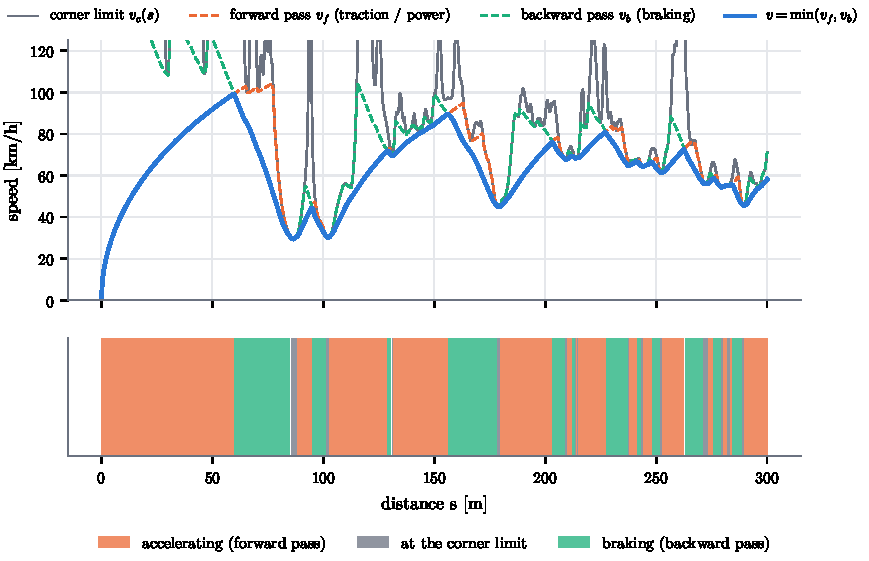
\includegraphics[width=\textwidth]{figures/pl_qss.pdf}
\caption{Construction of the QSS speed profile on the first \SI{300}{m} of the FSA 2025 autocross. The forward pass
(traction and power limited) and the backward pass (brake limited) are bounded by the corner speed $v_c$. Their
minimum is the result. Bottom: which limit is active along the track.}
\label{fig:qss}
\end{figure}

\subsection{Closed tracks}
For a closed track (skidpad circle, endurance), the start speed is not known. The curvature table is therefore
repeated three times and solved from standstill; the middle lap is the periodic flying-lap solution, and the
first lap gives the standing-start lap. Laps and timing modes are combined as follows:
\begin{equation}
T = \begin{cases} n_{laps}\,t_{lap} & \text{flying lap}\\ t_{first} + (n_{laps}-1)\,t_{lap} & \text{standing start}\\ t_{lap} & \text{single}\end{cases}
\end{equation}

\subsection{Signals and energy}
Along the profile, the solver also computes:
\begin{itemize}
  \item the accelerations $a_{x,j} = (v_{j+1}^2 - v_j^2)/(2\Delta s)$ and $a_{y,j} = v_j^2\kappa_j$;
  \item the wheel force $F_{x,j} = e_i m\,a_{x,j} + F_{res}(v_j)$ and the wheel power $P_{w,j} = F_{x,j}v_j$;
  \item the accumulator power
\begin{equation}
P_{b} = \begin{cases} P_w / (\eta_g\,\eta_m) & P_w\ge 0,\\ -\min(|P_w|, P_{regen})\,\eta_{regen} & P_w<0,\end{cases}
\label{eq:pbatt}
\end{equation}
        where the motor efficiency $\eta_m$ is constant or comes from a map
        $\eta_m(T_m, n_m)$ (\cref{sec:effmap}) with $T_m = F_x r_w/(i\eta_g)$ per motor set;
  \item the energy, by trapezoidal integration of $P_b$ over time.
\end{itemize}

\subsection{Cost}
The solver loops over $\approx\!10^4$ points per event with scalar arithmetic, specialised for the per-point
evaluation of \cref{eq:axacc,eq:axdec}. One evaluation of all four events, including the 16-lap endurance, takes
\SI{0.3}{s} on one CPU core.

%=====================================================================================================
\section{Tracks}\label{sec:tracks}
%=====================================================================================================
\paragraph{Basic tracks.} The acceleration track is a straight of \SI{75}{m}. The skidpad is a circle of radius
$R = 15.25/2 + 1.5 = \SI{9.125}{m}$ (the driven radius of the FS skidpad).

\paragraph{Curvature tables.} The FSA~2025 autocross and endurance tracks of the documentation are curvature
tables $(s, \kappa)$, with $x,y$ reconstructed by integration.

\paragraph{Measured coordinates.} The ``real'' tracks are measured $x,y$ coordinates. The LapSim method fits
not-a-knot cubic splines $x(s), y(s)$ in arc length (wrapped at the ends for a closed track). It evaluates the
curvature from the spline derivatives,
\begin{equation}
\kappa = \frac{x'y'' - y'x''}{(x'^2 + y'^2)^{3/2}},
\end{equation}
and smooths it with a moving mean over \SI{5}{m}. The filter width is a modelling choice with a large effect:
changing it moves the lap time by about $\pm6\,\%$.

\paragraph{Closure of curvature tables.} A curvature table integrated to $x,y$ generally does not close. The FSA
2025 endurance table ends \SI{17.3}{m} from its start. The QSS solver only uses $\kappa$, so this does not matter
there. A driven car (\cref{sec:transient}), however, would meet a jump. We therefore close the loop by spreading the
gap linearly along the lap:
\begin{equation}
\vect p_j \leftarrow \vect p_j - \frac{s_j}{L}\,\vect e,\qquad \vect e = \big(\vect p_{N-1} + (\vect p_{N-1}-\vect p_{N-2})\big) - \vect p_0,
\end{equation}
which changes the curvature by about $\SI{1}{cm}$ per metre of track, and leaves the heading at the join
unchanged (the heading mismatch of this table is zero).

%=====================================================================================================
\section{Competition model and scoring}\label{sec:scoring}
%=====================================================================================================
Each event has a track, a timing mode, a number of laps, a start speed and driver utilisation factors
(\cref{tab:events}).

\paragraph{Event vehicle.} The vehicle used for an event applies the utilisation factors. In endurance it also
applies the torque scale and the endurance power cap, $P = \min(P_{\max}, P_{\max}^{end})$ and
$T_{mot}\leftarrow s_T\,T_{mot}$.

\paragraph{Scoring.} The time $T$ is converted to points with the competition formula
\begin{equation}
\text{Points}(T) = P_{\min} + (P_{\max}-P_{\min})\left(\frac{T_{\max}-T}{T_{\max}-T_{\min}}\right)^{n},\qquad
T_{\min}\le T\le T_{\max},
\label{eq:score}
\end{equation}
clipped to $[P_{\min}, P_{\max}]$ outside that range. The parameters are those of the competition file
(\cref{tab:events}). The points cover the four dynamic events only. Efficiency and the static events are not
included, because the efficiency formula of the current rules was not available (the efficiency factor $T^2E$ is
reported, \cref{sec:energy}).

\begin{table}[t]
\centering\small
\caption{Events of \code{competition\_fsa2025.m} and the LR26 baseline result (QSS).}
\label{tab:events}
\setlength{\tabcolsep}{4.5pt}
\begin{tabular}{@{}lcccccccrr@{}}
\toprule
Event & Track & Laps & Timing & $u_x/u_y$ & $T_{\min}$ [s] & $T_{\max}$ [s] & $P_{\max}$, $n$ & $T$ [s] & Points\\
\midrule
Acceleration & \SI{75}{m} & 1 & single & 1.0/1.0 & 3.875 & 5.959 & 50, 2.12 & 4.662 & 19.88\\
Skidpad & $R=\SI{9.125}{m}$ & 1 & flying & 1.0/0.8 & 4.869 & 6.298 & 50, 2.19 & 5.154 & 31.65\\
Autocross & \SI{830}{m} & 1 & single & 0.9/0.8 & 42.65 & 63.92 & 100, 2.47 & 49.944 & 38.68\\
Endurance & \SI{1307.5}{m} & 16 & flying & 0.9/0.8 & 1253.2 & 1846.2 & 250, 2.46 & 1526.97 & 74.14\\
\midrule
\multicolumn{9}{@{}l}{Total of the dynamic events} & \textbf{164.35}\\
\bottomrule
\end{tabular}
\end{table}

%=====================================================================================================
\section{Analysis methods}\label{sec:studies}
%=====================================================================================================
A \emph{setup} is a list of parameter changes on top of \code{lr26\_params.m}. The forms are
\code{name=value}, \code{name*factor}, \code{name+delta} and \code{name-delta}, with the aliases of
\code{lts\_set\_param} (e.g.\ \code{mu} sets $\mu_y$ and keeps the ratio $\mu_x/\mu_y$); \code{<event>.util\_y=0.85}
changes a driver utilisation. Setups are stored as JSON and shared with the driverless simulator's dashboard.
Every study below is relative to the active setup.

\subsection{Sensitivity}
For each parameter $p$ with value $p_0$ and a relative step $\delta$ (default \SI{10}{\%}), the car is evaluated at
$(1\pm\delta)p_0$. As in the department's MATLAB method, the point sensitivity is linearised in the improving
direction:
\begin{equation}
S_P = \frac{\max\big(P(p_0(1+\delta)), P(p_0(1-\delta))\big) - P(p_0)}{100\,\delta}\quad[\text{points}/\%],
\end{equation}
together with the time change of each event in both directions. For mass, the sensitivity is also given per
kilogram, $S_P/(p_0\delta)$. A parameter whose value is zero (e.g.\ AWD off) cannot be scaled and is reported as
``no effect''.

\subsection{Sweeps and maps}
A sweep evaluates $n\le60$ absolute values of one parameter and records the total and every event's time, points
and energy, optionally with the speed traces of one event. A map does the same for a grid of two parameters (at
most $25\times25$) and reports the best point. A comparison evaluates up to eight setups. For each event, it gives
the speed traces and the time difference along the lap, $\Delta t(s) = t_k(s) - t_1(s)$, against the first setup.

%=====================================================================================================
\section{Energy and endurance}\label{sec:energy}
%=====================================================================================================
\subsection{Energy decomposition}
Over a flying lap the kinetic energy at start and end is equal, so the positive wheel work is spent on drag,
rolling resistance and braking:
\begin{equation}
\underbrace{\oint P_w^+\,dt}_{W_{drive}} = \underbrace{\oint F_D v\,dt}_{W_{drag}} + \underbrace{\oint (F_{res}-F_D) v\,dt}_{W_{roll}} + \underbrace{\oint P_w^-\,dt}_{W_{brake}},
\label{eq:balance}
\end{equation}
where $P_w^\pm$ are the positive and negative parts of the wheel power. The battery provides $W_{drive}$ plus the
drivetrain losses, and recuperation returns part of $W_{brake}$. \Cref{fig:energy} (right) shows the decomposition
of the LR26 endurance lap at the \SI{18}{kW} cap. Of the \SI{0.344}{kWh} drawn per lap, \SI{0.235}{kWh} (68\,\%)
end in the friction brakes, because recuperation is off in the baseline. Aerodynamic drag takes
\SI{0.054}{kWh}, the drivetrain \SI{0.050}{kWh} and rolling resistance \SI{0.006}{kWh}. \Cref{eq:balance} holds
numerically to 0.1\,\%, the trapezoidal integration error.

\subsection{Power cap for an energy budget}
The endurance is power limited by a cap $P_c$ (LR26: \SI{18}{kW}). The total endurance energy $E(P_c)$ grows
monotonically with the cap, so the largest cap whose energy fits a budget $E_b$,
\begin{equation}
P_c^\star = \max\{P_c\in[P_{lo}, P_{\max}] : E(P_c)\le E_b\},
\end{equation}
is found by bisection, to \SI{5}{W}. The tool also reports whether the budget limits the car at all, and whether
the lowest cap already exceeds it. A \SI{5.0}{kWh} budget gives $P_c^\star = \SI{15.3}{kW}$: an endurance time of
\SI{1549}{s} and 66.2 points, against 74.1 points with \SI{18}{kW} and \SI{5.5}{kWh}
(\cref{fig:energy}, left). The tool also reports the efficiency factor $EF = T^2E$.

\begin{figure}[t]
\centering
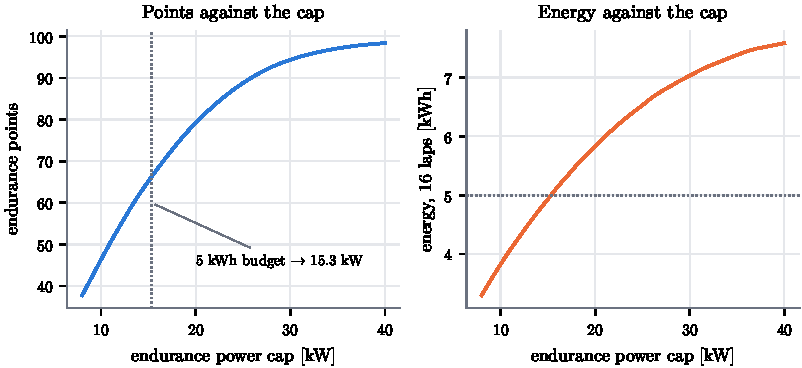
\includegraphics[width=\textwidth]{figures/pl_energy_cap.pdf}\\[2mm]
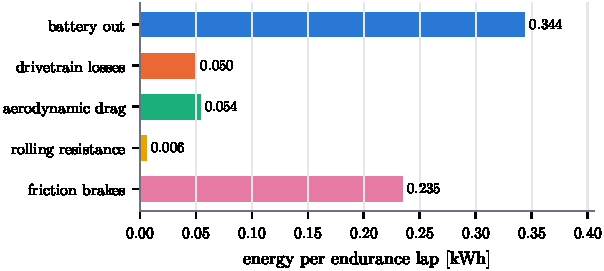
\includegraphics[width=0.62\textwidth]{figures/pl_energy_breakdown.pdf}
\caption{Top: endurance points and energy against the power cap. A \SI{5}{kWh} budget allows \SI{15.3}{kW}.
Bottom: energy of one endurance lap at the \SI{18}{kW} cap. Battery out = drivetrain losses + wheel work, and wheel
work = drag + rolling resistance + braking.}
\label{fig:energy}
\end{figure}

\subsection{Motor efficiency map}\label{sec:effmap}
The constant $\eta_m$ can be replaced by a map identified from inverter logs (\cref{sec:logs}). Per motor, the loss
model
\begin{equation}
P_{loss} = k_0 + k_1 T^2 + k_2 n + k_3 n^2\quad(n\text{ in krpm})
\end{equation}
is fitted by least squares to $P_{DC} - T\omega$. The map is then $\eta(T,n) = P_{mech}/(P_{mech}+P_{loss})$ on a
grid. It is bilinearly interpolated and clamped at the edges, with the axle torque shared equally by the motors of
a set. Outside the torque and speed range of the data, the $T^2$ term is an extrapolation, and the tool says so.

\subsection{ggV diagram}
For speeds $v_k$ and lateral accelerations from 0 to the steady-state limit $a_{y,\max}(v_k)$ (bisection on
$\mathcal F$), the drive and brake limits of \cref{eq:axacc,eq:axdec} form the ggV diagram (\cref{fig:ggv}). These
are exactly the limits the QSS solver uses, and the input that minimum-time and MPC planners need. For the LR26 at
the tyre limit:
\begin{itemize}
  \item the lateral limit grows from \SI{1.61}{g} at \SI{18}{km/h} to \SI{2.54}{g} at \SI{117}{km/h};
  \item the braking limit grows from \SI{1.46}{g} to \SI{2.77}{g};
  \item the drive limit falls from \SI{0.74}{g} to \SI{0.49}{g}. It is set by the motor torque
        (\SI{2.09}{kN} at the wheels, about what the rear tyres can transmit at low speed) and falls with
        aerodynamic drag.
\end{itemize}

\begin{figure}[t]
\centering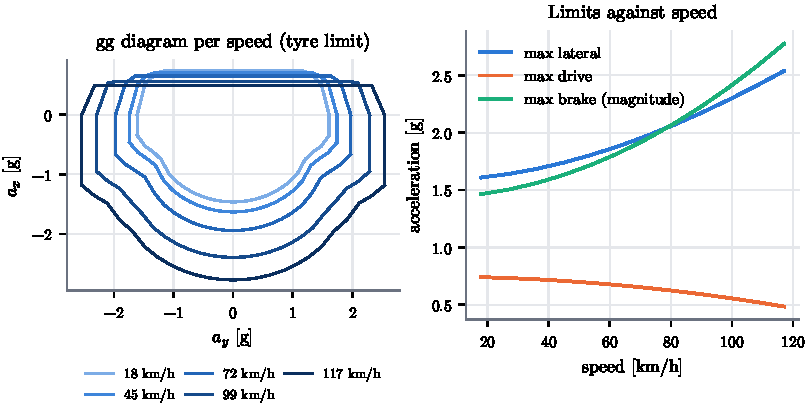
\includegraphics[width=\textwidth]{figures/pl_ggv.pdf}
\caption{ggV diagram of the LR26 at the tyre limit. Left: drive (upper) and brake (lower) limits against lateral
acceleration for five speeds. Right: the limits against speed. Downforce raises the lateral and braking limits; the
drive limit is set by the motor torque and falls with drag.}
\label{fig:ggv}
\end{figure}

%=====================================================================================================
\section{Transient lap}\label{sec:transient}
%=====================================================================================================
The QSS lap is an upper bound for a real car. Every point is at a limit, and there is no yaw, no steering, no
actuator delay and no tracking error. The transient lap measures how much of the QSS time a closed-loop driver can
actually achieve.

\paragraph{Vehicle.} The driverless simulator's dynamic single-track model in performance mode~\cite{dvsim}: the
same wheel loads, potentials, friction ellipse, powertrain, brakes and aerodynamics as \cref{sec:model}, applied
to axle forces with a Magic-Formula slip-angle shape~\cite{pacejka2012}. On top come a yaw inertia ($I_z =
\SI{120}{kg\,m^2}$), a steering actuator with rate limit, and longitudinal and steering lags. The event vehicle
(endurance torque scale and power cap included) is used at the tyre limit ($u_x=u_y=1$): utilisation is a driver
property and is passed to the driver.

\paragraph{Driver.} The simulator's reference driver: pure pursuit on the event's centre line, with a speed target
from the QSS profile at grip utilisation $u_y$ and longitudinal utilisation $u_x/u_y$, tracked by a proportional
controller (details in~\cite{dvsim}). For an open track, the reference path gets a run-up of \SI{5}{m} behind the
start line, so the target speed at the line is not zero.

\paragraph{Procedure.} The model is integrated with RK4 (sub-steps $\le\SI{2}{ms}$) at a control period of
\SI{20}{ms}.
\begin{itemize}
  \item \textbf{Progress.} Progress along the path is the projection of the car onto the polyline, searched near
        the last index. Laps are counted on closed tracks, and the signed lateral offset is recorded.
  \item \textbf{Closed tracks.} The car drives two laps from standstill. Lap crossings are interpolated within a
        step, and the second lap is the flying lap.
  \item \textbf{Open tracks.} The run ends at the track's end, with the crossing interpolated.
\end{itemize}
Time, points, top speed, sideslip, steering, lateral offset, time spent more than half a track width from the line,
and energy are recorded. The time lost to QSS along the lap is
\begin{equation}
\Delta t(s) = t_{tr}(s) - t_{QSS}(s).
\end{equation}

\paragraph{Results.} \Cref{tab:transient,fig:transient} show the baseline. The transient times are 3.5\,\%
(acceleration), 4.3\,\% (skidpad), 7.5\,\% (autocross) and 4.8\,\% (endurance lap) above QSS. On the autocross the
loss accumulates steadily: the driver brakes earlier and does not reach the QSS apex speeds (top speed
\SI{104}{km/h} against \SI{118}{km/h}). Sideslip stays below \ang{4.5} and the lateral offset below \SI{0.52}{m},
with no time off track. The transient endurance lap uses 36\,\% less energy than QSS
(\SI{0.220}{kWh} against \SI{0.344}{kWh}), because the driver cruises below the power cap where QSS accelerates at
it. This is a property of the driver, not of the car.

\begin{table}[t]
\centering\small
\caption{Transient lap (dynamic model + reference driver) against QSS, LR26 baseline, FSA~2025 tracks
(documentation version). Endurance: lap time of the flying lap.}
\label{tab:transient}
\setlength{\tabcolsep}{4pt}
\begin{tabular}{@{}lccccccc@{}}
\toprule
Event & QSS & Transient & $\Delta$ & $v_{\max}$ QSS / tr. & $\beta_{\max}$ & Offset$_{\max}$ & Compute\\
 & [s] & [s] & & [km/h] & [deg] & [m] & [s]\\
\midrule
Acceleration & 4.662 & 4.825 & +3.5\,\% & 109.3 / 102.7 & 0.0 & 0.00 & 0.4\\
Skidpad & 5.154 & 5.375 & +4.3\,\% & 40.0 / 38.5 & 3.7 & 0.10 & 0.6\\
Autocross & 49.944 & 53.712 & +7.5\,\% & 117.9 / 103.7 & 3.8 & 0.51 & 3.2\\
Endurance lap & 95.435 & 100.000 & +4.8\,\% & 80.2 / 74.9 & 4.5 & 0.36 & 11.6\\
\bottomrule
\end{tabular}
\end{table}

\begin{figure}[t]
\centering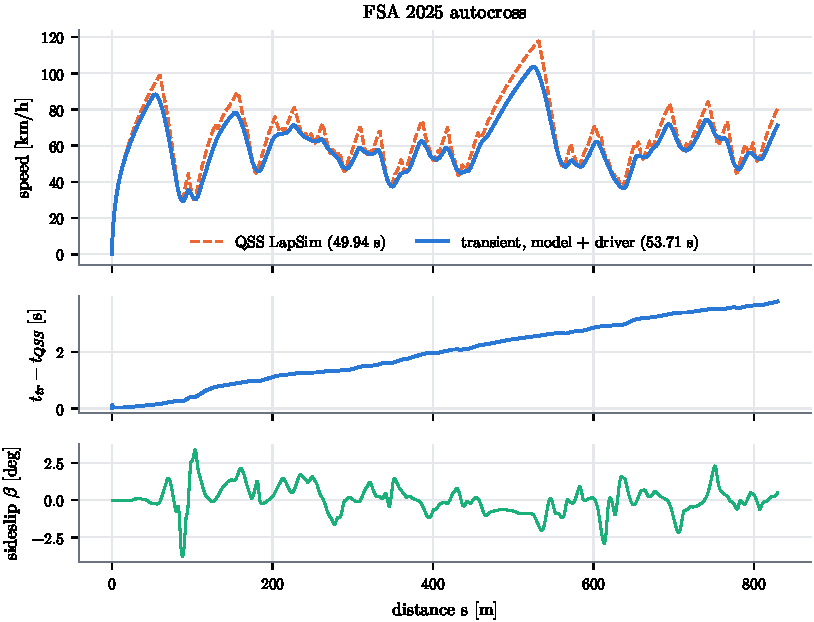
\includegraphics[width=\textwidth]{figures/pl_transient.pdf}
\caption{Transient lap against QSS on the FSA 2025 autocross. Top: speed. Middle: time lost to QSS along the lap.
Bottom: sideslip angle of the dynamic model.}
\label{fig:transient}
\end{figure}

On the ``real'' FSA 2025 tracks, the transient endurance lap is \SI{112}{s} against \SI{96}{s}. The driver derives
its speed targets from the unfiltered $x,y$ points, while LapSim filters the curvature over \SI{5}{m}. Until the
driver uses the filtered curvature, transient-against-QSS comparisons should be made on the documentation tracks.

%=====================================================================================================
\section{Lap time methods}\label{sec:methods}
%=====================================================================================================
QSS answers ``which setup is faster'' quickly, but it fixes the line and ignores yaw, steering and the shape of the
tyre curve. The Lab therefore solves the same car with further methods, so that each question is answered by the
simplest method that contains the physics it depends on (\cref{tab:methodguide}). Implementation:
\code{perf/perflab/ocp.py} and \code{methods.py}; the full description, with every hypothesis, is
\code{docs/PERF\_METHODS.md}.

\begin{table}[t]
\centering\small
\caption{Which method for which question.}\label{tab:methodguide}
\begin{tabularx}{\textwidth}{@{}>{\raggedright\arraybackslash}X>{\raggedright\arraybackslash}p{4.3cm}@{}}
\toprule
Question & Method\\
\midrule
Ranking of changes, sensitivities, sweeps & LapSim QSS (\cref{sec:solver})\\
Is a gain larger than the parameter uncertainty? & Monte-Carlo on QSS (\cref{sec:mc})\\
Is the QSS solver the limit? & OCP point mass, fixed line\\
Yaw inertia, steering limits, tyre shape, balance & OCP single / double track\\
Torque vectoring & OCP double track with free wheel forces\\
Behaviour with a driver, stability & transient lap (\cref{sec:transient})\\
Racing line on a known width & OCP with free line (true centre lines only)\\
\bottomrule
\end{tabularx}
\end{table}

\subsection{Minimum-time optimal control}
The optimal lap of a perfect driver is the solution of~\cite{casanova2000,perantoni2014,lot2014}
\begin{equation}
\min_{\mathbf{x}(s),\,\mathbf{u}(s)} \; T=\int_0^{L}\frac{\mathrm{d}s}{\dot s}
\quad\text{s.t.}\quad \mathbf{x}'=\frac{\mathbf{f}(\mathbf{x},\mathbf{u})}{\dot s},\;
\mathbf{g}(\mathbf{x},\mathbf{u})\le 0,\; |n|\le \tfrac{w-b}{2}\ \text{or}\ n=0,
\label{eq:ocp}
\end{equation}
in curvilinear coordinates: $s$ along the event's line, the lateral offset $n$ and the heading $\xi$ of the car
relative to the line, with
\begin{equation}
\dot s=\frac{v_x\cos\xi-v_y\sin\xi}{1-n\kappa},\qquad \dot n=v_x\sin\xi+v_y\cos\xi,\qquad \dot\xi=r-\kappa\dot s .
\end{equation}
The problem is discretised on a uniform \SI{1}{m} grid (curvature averaged per metre) by trapezoidal collocation;
closed tracks are periodic (flying lap). CasADi~\cite{casadi2019} builds it with exact derivatives and IPOPT~\cite{ipopt2006}
solves it. Each model starts from the solution of the simpler one: QSS speeds $\to$ point mass $\to$ single track
$\to$ double track. A stage that does not converge returns no time. Tyre potentials, load sensitivity, load transfer,
aerodynamics, resistance, powertrain limits and the event's utilisation are those of \cref{sec:model}; yaw inertia,
steering limits and the Magic-Formula shape come from the simulator's vehicle file, as for the transient lap.

\paragraph{Point mass.} States $n,\xi,v$; inputs $a_x$ and the path curvature $\kappa_p$, constant per interval.
The combined limit is a smooth envelope fitted to the ggV of \cref{sec:model},
$(|a_y|/a_{y,\max}(v))^{p}+(a_x/a_{\lim}(v))^{p}\le1$, with quadratic $a_{y,\max}$, $a_{\lim}$ and separate exponents
for braking and traction (fitted: 1.90 and 2.10); motor force, power and speed limits are exact constraints. With
inputs at the nodes the path curvature zig-zags around $\kappa$ and beats the envelope; constant inputs per
interval, with the limits at both ends, remove this.

\paragraph{Single track.} States $n,\xi,v_x,v_y,r,\delta$; inputs the steering rate and the axle longitudinal
forces; the accelerations $a_x,a_y$ are algebraic variables that set the quasi-static wheel loads. Lateral forces
follow the Magic-Formula shape~\cite{pacejka2012} scaled by the axle potential, combined by
$(F_x/F_{x,\max})^2+(F_y/F_{y,\max})^2\le1$; $|\delta|$ and $|\dot\delta|$ are limited.

\paragraph{Double track.} Four wheels, each with its slip angle, load, potential and friction ellipse. Without torque
vectoring the left and right forces of an axle are equal; with it they are free within the per-motor limit.

\paragraph{Results.} \Cref{tab:ocp,fig:methods}. With the fixed line the point-mass OCP agrees with QSS on the same grid
within \SI{0.3}{\%}: LapSim's passes find the optimum of its own model. The dynamic models are 1.5--5\,\% slower than
QSS: yaw and steering take time, and the tyre curve falls beyond its peak. They are close to the transient lap,
which is driven at the event's utilisation. Torque vectoring recovers what lateral load transfer costs the double
track (\SI{2.0}{s} on autocross). A free line is only meaningful on a true centre line: the FSA tables are already a
driven line, and re-optimising them within \SI{3.5}{m} gives a 24\,\% faster endurance lap, an artefact.

\begin{table}[t]
\centering\small
\caption{Event times of the methods, LR26 baseline, fixed line (endurance: one lap). Compute times on one
core.}\label{tab:ocp}
\begin{tabular}{@{}lrrrrr@{}}
\toprule
 & Acceleration & Skidpad & Autocross & Endurance lap & Compute\\
\midrule
LapSim QSS & 4.662 & 5.154 & 49.94 & 95.44 & \SI{0.2}{s}\\
QSS on the \SI{1}{m} grid & 4.662 & 5.154 & 49.85 & 94.47 & --\\
QSS point mass (friction circle) & 4.704 & 5.010 & 50.92 & 97.61 & \SI{0.03}{s}\\
Transient lap & 4.83 & 5.38 & 53.71 & 100.0 & 0.2--\SI{10}{s}\\
OCP point mass & 4.669 & 5.142 & 49.79 & 94.21 & 0.1--\SI{2}{s}\\
OCP single track & 4.662 & 5.231 & 52.09 & 99.97 & up to \SI{40}{s}\\
OCP double track & 4.662 & 5.398 & 54.03 & 102.72 & up to \SI{50}{s}\\
OCP double track + TV & -- & 5.282 & 52.07 & -- & up to \SI{65}{s}\\
\bottomrule
\end{tabular}
\end{table}

\begin{figure}[t]
\centering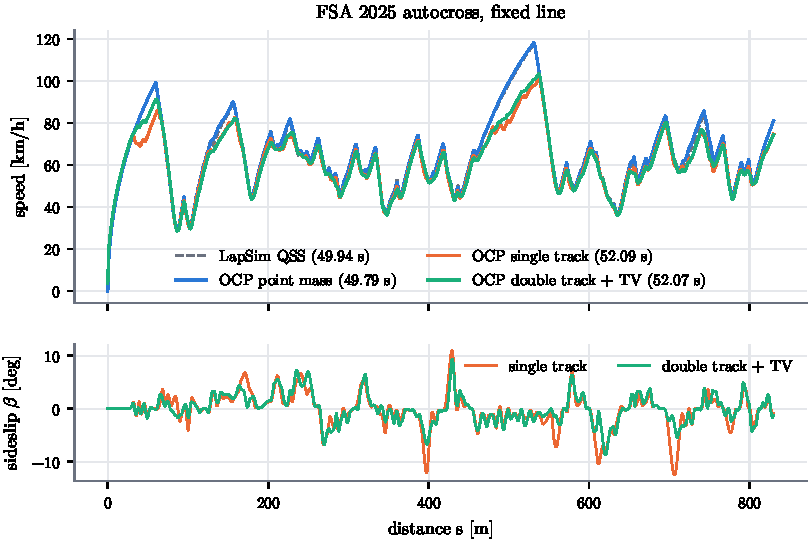
\includegraphics[width=\textwidth]{figures/pl_methods_autocross.pdf}
\caption{FSA 2025 autocross: speed of LapSim QSS and of the OCP models (top), sideslip of the dynamic models
(bottom).}
\label{fig:methods}
\end{figure}

\subsection{Method comparison}
For a decision the question is not the absolute time but the time change of a setup change, and whether the methods
agree on it. On the skidpad, \SI{5}{kg} less mass gains between \SI{6.3}{ms} (double track) and \SI{9.8}{ms}
(friction circle), \SI{8.1}{ms} with QSS: every method agrees on the sign, and the spread ($\pm20\,\%$) is the
model uncertainty of the gain. The Methods page runs this comparison for any event and change.

\subsection{Robustness}\label{sec:mc}
The parameters are uncertain. The Monte-Carlo study multiplies each uncertain parameter by $1+\sigma z$,
$z\sim\mathcal N(0,1)$ clipped at $\pm3$ (default $\sigma$: friction 3\,\%, mass 1\,\%, $c_z$ and $c_w$ 5\,\%, power
2\,\%, lateral utilisation 2\,\%), runs QSS for every draw and, for a change, the same draws again (paired samples).
For the baseline the total has $\sigma\approx19$ points: the scoring is steep near the reference times. The paired
gain of \SI{5}{kg} less is $3.9\pm0.3$ points and positive in every draw (\cref{fig:mc}). A change is worth it when
the methods agree on its sign and the probability of a gain is high.

\begin{figure}[t]
\centering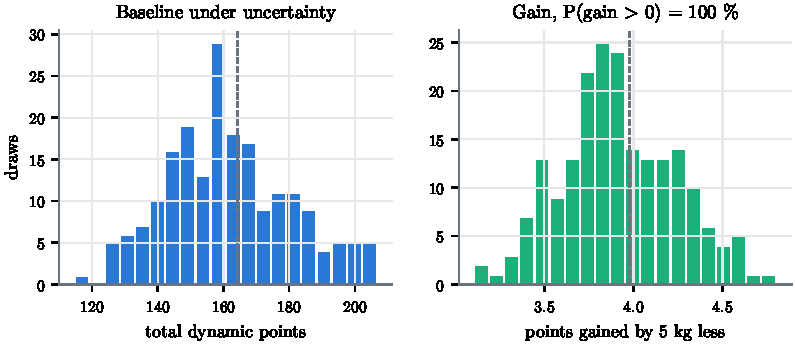
\includegraphics[width=\textwidth]{figures/pl_montecarlo.pdf}
\caption{Monte-Carlo, 200 draws: total dynamic points of the baseline (left) and points gained by \SI{5}{kg} less on
the same draws (right). Dashed: nominal parameters.}
\label{fig:mc}
\end{figure}

%=====================================================================================================
\section{Log correlation}\label{sec:logs}
%=====================================================================================================
\subsection{Speed and acceleration traces}
A log (MF4, read with an own MDF~4 parser, or CSV) provides speed and, optionally, longitudinal and lateral
acceleration, in selectable units. Speed may also come from motor speed, $v = n\,r_w\,2\pi/(60\,i)$. That is only
the vehicle speed while the wheels roll on the road, which the roll-out check below tests. Signals are resampled to
\SI{20}{Hz} (zero-order hold) and cut to a time window.

\paragraph{Alignment.} Logs and simulation are compared on distance, not time, because time accumulates
differences. The log distance is $s(t) = \int v\,dt$ (or a distance column), shifted by an offset $s_0$ for the
difference between timing line and log start. The offset is either given or found by a grid search:
\begin{equation}
s_0^\star = \arg\min_{s_0\in[-30,30]\,\si{m}} \operatorname{RMSE}\big(v_{log}(s+s_0),\, v_{sim}(s)\big).
\end{equation}

\paragraph{Metrics.} Over the common distance range, the tool reports the speed RMSE and bias (log minus
simulation), the RMSE of $a_x$ and $|a_y|$, the times over the compared part, and the time difference along the
lap. This follows the correlation metric proposed in the team documentation.

\paragraph{Check against the documentation trace.} LR26\_LapSim ships the speed trace of the documentation's own
Python LTS on the FSA 2025 autocross. Against it, the port gives a speed RMSE of \SI{3.2}{km/h}, a bias of
\SI{-0.07}{km/h} and a time difference of \SI{-2.6}{ms} over the lap, with a searched offset of \SI{1.5}{m}
(\cref{fig:corr}). On the endurance, the RMSE is \SI{4.3}{km/h} and the time difference \SI{0.28}{s}. The remaining
difference is concentrated at the highest speeds, where the documentation's model reaches 4~km/h less.

\begin{figure}[t]
\centering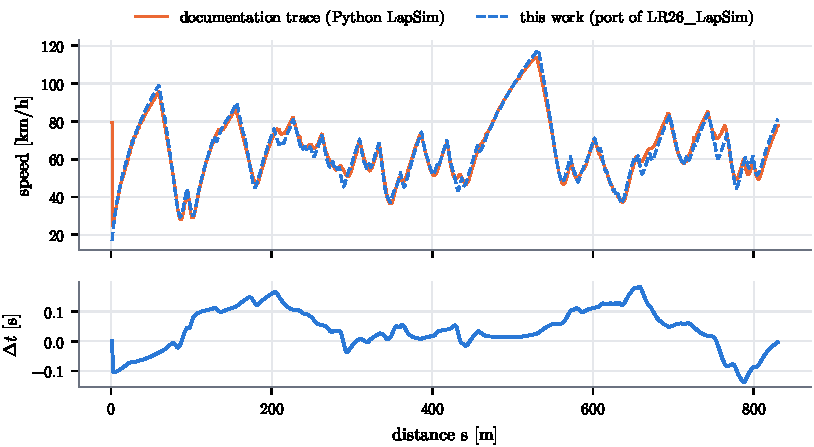
\includegraphics[width=\textwidth]{figures/pl_correlation.pdf}
\caption{Correlation of the port with the speed trace of the documentation's Python LTS (FSA 2025 autocross).
Bottom: time difference along the lap (reference minus port).}
\label{fig:corr}
\end{figure}

\subsection{Powertrain from inverter logs}
From the LR26 inverter channels (speed, torque and DC power of both drive units), driving samples with torque
$>\SI{0.3}{Nm}$ and DC power $>\SI{0.5}{kW}$ give the efficiency
\begin{equation}
\eta = \frac{T\,\omega}{P_{DC}}.
\end{equation}
The median efficiency is reported per torque--speed bin (bins with at least 20 samples), together with the
least-squares loss model of \cref{sec:effmap}.

\paragraph{Roll-out check.} The tool measures the median deceleration in the zero-torque, no-throttle, no-brake
stretches. A car rolling on the road decelerates at a few tenths of \si{m/s^2}. A value above
\SI{0.6}{m/s^2} indicates a stand or dyno, and the log must not be used to fit vehicle dynamics. The team's only
log so far (D1F58) fails this check and has no GPS or IMU, so vehicle-level correlation with the real car is still
open.

%=====================================================================================================
\section{Results of the analyses}\label{sec:results}
%=====================================================================================================
\paragraph{Sensitivities.} \Cref{fig:sens,tab:sens} rank the parameters by $S_P$:
\begin{itemize}
  \item \textbf{Friction} dominates with 5.6 points/\%. A 10\,\% loss of grip costs 50 points, 2.7~s in autocross
        and 70~s in endurance.
  \item \textbf{Mass} follows with 2.5 points/\% (0.86 points/kg, \SI{32}{ms/kg} in autocross).
  \item \textbf{Motor torque and gear ratio} act identically (0.89 points/\%). Both scale the wheel force below
        the power limit, which binds only in acceleration and autocross.
  \item \textbf{Aerodynamics.} $c_z$ is worth 0.50 points/\%, and moving the aero balance rearwards helps
        (0.34 points/\%). The rear axle limits every corner, so it needs more of the downforce.
  \item \textbf{No effect.} $P_{\max}$ has no effect: with \SI{38}{Nm} the motor reaches \SI{80}{kW} only at
        about \SI{131}{km/h}, close to the top speed of \SI{136}{km/h} that no event reaches, and the endurance
        has its own cap.
\end{itemize}

\begin{figure}[t]
\centering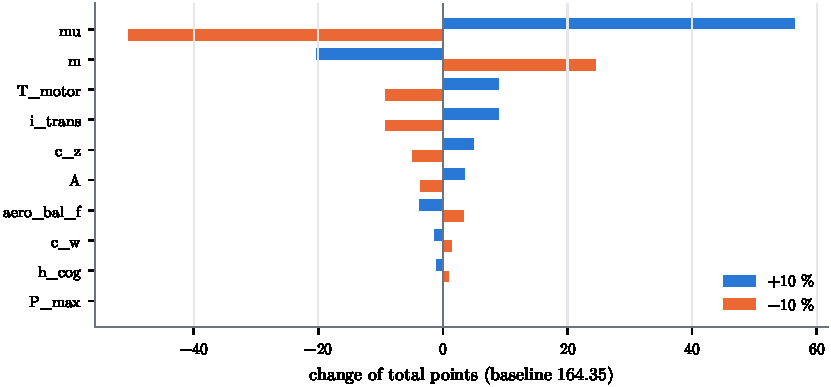
\includegraphics[width=\textwidth]{figures/pl_sensitivity.pdf}
\caption{Change of the total dynamic points for $\pm10\,\%$ of each parameter, LR26 baseline (164.35 points).}
\label{fig:sens}
\end{figure}

\begin{table}[t]
\centering\small
\caption{Sensitivities of the LR26 (QSS, $\delta = \SI{10}{\%}$): points per \% in the improving direction and
time change per event for $+10\,\%$.}
\label{tab:sens}
\begin{tabular}{@{}lrrcrrrr@{}}
\toprule
Parameter & Value & P/\% & better & $\Delta T_{acc}$ [s] & $\Delta T_{skid}$ [s] & $\Delta T_{AX}$ [s] & $\Delta T_{end}$ [s]\\
\midrule
$\mu$ & 1.64 & 5.643 & $+$ & 0.000 & $-0.256$ & $-2.261$ & $-58.30$\\
$m$ & 284 & 2.451 & $-$ & $+0.216$ & $+0.044$ & $+0.842$ & $+21.00$\\
$T_{mot}$ & 38 & 0.891 & $+$ & $-0.218$ & 0.000 & $-0.350$ & 0.00\\
$i$ & 14.5 & 0.891 & $+$ & $-0.218$ & 0.000 & $-0.350$ & 0.00\\
$c_z$ & 4.15 & 0.495 & $+$ & 0.000 & $-0.020$ & $-0.306$ & $-5.08$\\
$A$ & 1.044 & 0.352 & $+$ & $+0.014$ & $-0.020$ & $-0.251$ & $-3.31$\\
$k_f$ & 0.485 & 0.338 & $-$ & 0.000 & $+0.019$ & $+0.224$ & $+3.82$\\
$c_w$ & 1.38 & 0.136 & $-$ & $+0.014$ & 0.000 & $+0.051$ & $+1.76$\\
$h$ & 0.265 & 0.089 & $-$ & 0.000 & $+0.012$ & $+0.014$ & $+0.76$\\
$P_{\max}$ & 80\,000 & 0.000 & -- & 0.000 & 0.000 & 0.000 & 0.00\\
\bottomrule
\end{tabular}
\end{table}

\paragraph{Gear ratio.} \Cref{fig:gear} sweeps the gear ratio from 11.6 to 23.2:
\begin{itemize}
  \item The total peaks at $i\approx19.3$ with 185.8 points, 21.4 points above the baseline of 14.5. Almost all of
        the gain comes from the acceleration (points rising steeply with torque at the wheel) and the autocross.
  \item The endurance is insensitive, because it is power capped.
  \item Above $i\approx19$, the top speed $v_{\max}$ falls below the speeds the car reaches, and the acceleration
        and autocross points drop.
\end{itemize}
This agrees with the documentation's study (Table~2.2: $i=19$ gives 183.6 points).

\begin{figure}[t]
\centering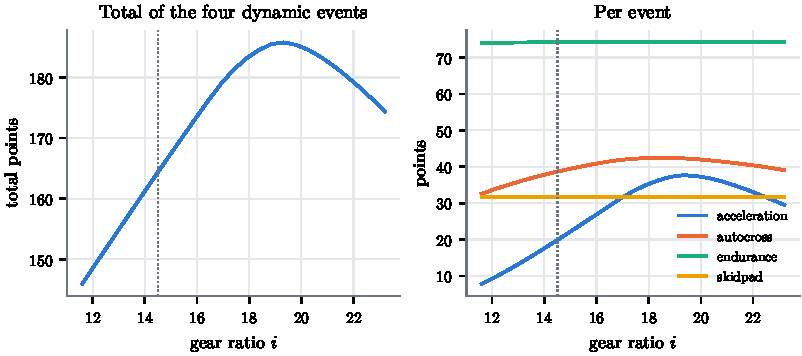
\includegraphics[width=\textwidth]{figures/pl_sweep_gear.pdf}
\caption{Gear ratio sweep. Left: total points (dotted: LR26, $i=14.5$). Right: points per event.}
\label{fig:gear}
\end{figure}

\paragraph{Aerodynamic trade-off.} \Cref{fig:aero} maps the total over $c_z$ and $c_w$. The iso-point lines are
nearly straight with a slope of about one: around the LR26, $+0.1$ in $c_z$ gains 1.19 points and $+0.1$ in $c_w$
loses 0.99 points. An aerodynamic change therefore pays off as long as it adds less than about 1.2 units of $c_w$
per unit of $c_z$.

\begin{figure}[t]
\centering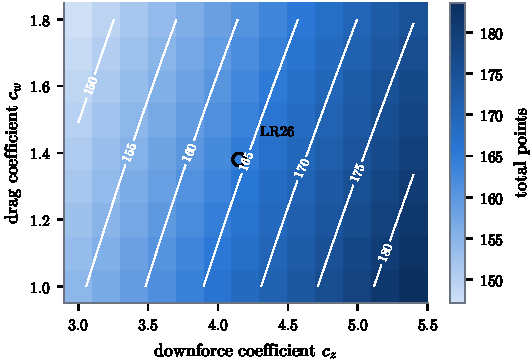
\includegraphics[width=0.62\textwidth]{figures/pl_map_aero.pdf}
\caption{Total points over the downforce and drag coefficients (circle: LR26).}
\label{fig:aero}
\end{figure}

\paragraph{Model order.} A point-mass solver without load transfer, registered as a plug-in solver, gives 154.24
points. The axle model with load transfer gives 164.35. The load transfer matters mainly in the endurance
(\SI{1561.7}{s} against \SI{1527.0}{s}) and in the autocross.

\paragraph{Real tracks.} The measured FSA 2025 tracks give 163.32 points:
\begin{itemize}
  \item autocross \SI{49.26}{s} (documentation \SI{49.94}{s});
  \item endurance lap \SI{96.33}{s} (\SI{95.44}{s}).
\end{itemize}

%=====================================================================================================
\section{Software}\label{sec:software}
%=====================================================================================================
The Performance Lab is a single-page web application served by a standard-library HTTP server on
\code{127.0.0.1:8090}. A double-click on \code{perf.bat} finds Python $\ge3.9$, asks before installing numpy,
scipy and pyyaml (and the optional CasADi for the optimal-control models), and opens the browser.
\begin{itemize}
  \item \textbf{Model.} The model code is the driverless simulator's \code{fsdsim.perf} package, imported
        unchanged.
  \item \textbf{Jobs.} Long studies run one at a time on a background worker, with progress and cancellation.
        The global efficiency-map selection is protected by a lock.
  \item \textbf{Front end.} The charts are own SVG code (no external libraries, works offline), with a validated
        colour-blind-safe palette and hover read-outs. Every result exports to CSV.
  \item \textbf{Security.} POST requests require a custom header that other web pages cannot send without CORS.
        Uploads are restricted to \code{.mf4}/\code{.csv} names in one folder, and path traversal is rejected.
\end{itemize}
The MATLAB files are only read, and re-read when they change.

%=====================================================================================================
\section{Verification}\label{sec:verification}
%=====================================================================================================
\begin{itemize}
  \item \textbf{Port against MATLAB.} Against the results of the MATLAB LapSim for 10 swept parameters (85
        values, all four events), the largest time difference is below \SI{0.005}{ms}, the rounding of the
        stored results. The baseline is reproduced exactly: \SI{4.662}{s}, \SI{5.154}{s}, \SI{49.944}{s},
        \SI{1526.97}{s}, 164.35 points.
  \item \textbf{Unit tests.} 23 tests cover the application:
        \begin{itemize}
          \item the identity of its runs with the port;
          \item parameter validation;
          \item the sign and order of sensitivities;
          \item the energy balance of \cref{eq:balance}, and that the power cap meets the budget;
          \item the loop closure;
          \item transient runs within bounds of QSS;
          \item offset recovery in correlation (a lap shifted by \SI{12}{m} is found to within \SI{1}{m});
          \item efficiency identification from a synthetic MF4 log;
          \item background jobs and the HTTP interface;
          \item the OCP: point mass within \SI{0.5}{\%} of QSS on the same grid, the dynamic models converge and are
                not faster than the point mass, torque vectoring is not slower, a failed stage gives no time;
          \item the method comparison and the Monte-Carlo study (reproducible draws, paired gains).
        \end{itemize}
        Together with the rest of the project, 335 tests pass.
  \item \textbf{Platform.} The application was verified with Python 3.9 and 3.13. The Windows start script and
        its pip step are written for \code{cmd} and still need to be run on a Windows PC.
\end{itemize}

%=====================================================================================================
\section{Limitations}\label{sec:limits}
%=====================================================================================================
\begin{itemize}
  \item \textbf{QSS assumptions.} QSS assumes the car is always at a limit, on a fixed line, with no yaw or
        transient tyre behaviour. The transient lap bounds the resulting error for the reference driver (3.5--8\,\%)
        but uses the same line.
  \item \textbf{Fixed path.} The path is the track file's line. The OCP can optimise the line, but should not be
        applied to the measured tracks, which are already a driven line.
  \item \textbf{OCP.} The optimal-control models assume a perfect driver, quasi-static load transfer and no tyre
        relaxation; yaw inertia and the tyre shape are less well known than the LapSim parameters. They were checked
        against QSS and the transient lap, not against car data.
  \item \textbf{Model choices.} The lateral load transfer distribution, aero efficiency and tyre load sensitivity
        are model assumptions of the LR26 set, and should be identified on the car.
  \item \textbf{Scoring.} Scoring covers the dynamic events only; efficiency points are missing until the current
        rule formula is available.
  \item \textbf{Correlation data.} Vehicle-level correlation needs a log with GPS or IMU speed on the road, which
        the team does not have yet.
\end{itemize}

%=====================================================================================================
\section{Conclusion}
%=====================================================================================================
The Performance Lab makes the LR26 lap time simulation available as a verified, stand-alone tool. It reproduces the
MATLAB model exactly, evaluates a setup in \SI{0.3}{s}, and adds the analyses a performance evaluation needs:
sensitivities, sweeps, comparisons, energy, ggV, a transient check of the QSS result, and correlation with data.

On the baseline car, the analyses point to three levers:
\begin{itemize}
  \item tyre grip and mass;
  \item a shorter gearing, where $i\approx19$ is worth about 21 points;
  \item downforce, which pays off whenever it costs less than about 1.2 units of $c_w$ per unit of $c_z$.
\end{itemize}
Recuperation would recover part of the 68\,\% of endurance energy currently dissipated in the brakes.

%=====================================================================================================
\begin{thebibliography}{99}\small
\bibitem{dvsim} Lions Racing Team, ``fsg-dv-sim: A shared-model simulation environment for the Lions Racing LR26
Formula Student driverless vehicle,'' technical report, Nov.~2026 (companion report, \code{docs/paper}).
\bibitem{siegler2000} B.~Siegler, A.~Deakin, D.~Crolla, ``Lap time simulation: Comparison of steady state,
quasi-static and transient racing car cornering strategies,'' SAE Technical Paper 2000-01-3563, 2000.
\bibitem{brayshaw2005} D.~L.~Brayshaw, M.~F.~Harrison, ``A quasi steady state approach to race car lap simulation
in order to understand the effects of racing line and centre of gravity location,'' \emph{Proc.\ IMechE Part~D:
J.\ Automobile Engineering}, vol.~219, no.~6, pp.~725--739, 2005.
\bibitem{casanova2000} D.~Casanova, ``On minimum time vehicle manoeuvring: The theoretical optimal lap,''
PhD thesis, Cranfield University, 2000.
\bibitem{pacejka2012} H.~B.~Pacejka, \emph{Tire and Vehicle Dynamics}, 3rd~ed. Butterworth-Heinemann, 2012.
\bibitem{milliken1995} W.~F.~Milliken, D.~L.~Milliken, \emph{Race Car Vehicle Dynamics}. SAE International, 1995.
\bibitem{perantoni2014} G.~Perantoni, D.~J.~N.~Limebeer, ``Optimal control for a Formula One car with variable
parameters,'' \emph{Vehicle System Dynamics}, vol.~52, no.~5, pp.~653--678, 2014.
\bibitem{lot2014} R.~Lot, F.~Biral, ``A curvilinear abscissa approach for the lap time optimization of racing
vehicles,'' \emph{IFAC Proceedings Volumes}, vol.~47, no.~3, pp.~7559--7565, 2014.
\bibitem{casadi2019} J.~A.~E.~Andersson, J.~Gillis, G.~Horn, J.~B.~Rawlings, M.~Diehl, ``CasADi: a software
framework for nonlinear optimization and optimal control,'' \emph{Mathematical Programming Computation}, vol.~11,
pp.~1--36, 2019.
\bibitem{ipopt2006} A.~W\"achter, L.~T.~Biegler, ``On the implementation of an interior-point filter line-search
algorithm for large-scale nonlinear programming,'' \emph{Mathematical Programming}, vol.~106, pp.~25--57, 2006.
\bibitem{rajamani2012} R.~Rajamani, \emph{Vehicle Dynamics and Control}, 2nd~ed. Springer, 2012.
\end{thebibliography}

\appendix
\section{Reproducing the results}
\begin{itemize}[before=\sloppy]
  \item All figures and numbers: \code{python3 docs/paper/figures/make\_figures.py} (writes \code{numbers.json}).
  \item The application: \code{perf\textbackslash perf.bat} on Windows, or \code{python perf/app.py}.
  \item Section~\ref{sec:methods} only: \code{make\_figures.py methods}.
  \item Tests: \code{python3 -m unittest tests.test\_perf\_app tests.test\_perf\_ocp}.
\end{itemize}

\end{document}
